% Options for packages loaded elsewhere
\PassOptionsToPackage{unicode}{hyperref}
\PassOptionsToPackage{hyphens}{url}
\PassOptionsToPackage{dvipsnames,svgnames,x11names}{xcolor}
%
\documentclass[
  letterpaper,
  DIV=11,
  numbers=noendperiod]{scrartcl}

\usepackage{amsmath,amssymb}
\usepackage{iftex}
\ifPDFTeX
  \usepackage[T1]{fontenc}
  \usepackage[utf8]{inputenc}
  \usepackage{textcomp} % provide euro and other symbols
\else % if luatex or xetex
  \usepackage{unicode-math}
  \defaultfontfeatures{Scale=MatchLowercase}
  \defaultfontfeatures[\rmfamily]{Ligatures=TeX,Scale=1}
\fi
\usepackage{lmodern}
\ifPDFTeX\else  
    % xetex/luatex font selection
\fi
% Use upquote if available, for straight quotes in verbatim environments
\IfFileExists{upquote.sty}{\usepackage{upquote}}{}
\IfFileExists{microtype.sty}{% use microtype if available
  \usepackage[]{microtype}
  \UseMicrotypeSet[protrusion]{basicmath} % disable protrusion for tt fonts
}{}
\makeatletter
\@ifundefined{KOMAClassName}{% if non-KOMA class
  \IfFileExists{parskip.sty}{%
    \usepackage{parskip}
  }{% else
    \setlength{\parindent}{0pt}
    \setlength{\parskip}{6pt plus 2pt minus 1pt}}
}{% if KOMA class
  \KOMAoptions{parskip=half}}
\makeatother
\usepackage{xcolor}
\setlength{\emergencystretch}{3em} % prevent overfull lines
\setcounter{secnumdepth}{5}
% Make \paragraph and \subparagraph free-standing
\ifx\paragraph\undefined\else
  \let\oldparagraph\paragraph
  \renewcommand{\paragraph}[1]{\oldparagraph{#1}\mbox{}}
\fi
\ifx\subparagraph\undefined\else
  \let\oldsubparagraph\subparagraph
  \renewcommand{\subparagraph}[1]{\oldsubparagraph{#1}\mbox{}}
\fi

\usepackage{color}
\usepackage{fancyvrb}
\newcommand{\VerbBar}{|}
\newcommand{\VERB}{\Verb[commandchars=\\\{\}]}
\DefineVerbatimEnvironment{Highlighting}{Verbatim}{commandchars=\\\{\}}
% Add ',fontsize=\small' for more characters per line
\usepackage{framed}
\definecolor{shadecolor}{RGB}{241,243,245}
\newenvironment{Shaded}{\begin{snugshade}}{\end{snugshade}}
\newcommand{\AlertTok}[1]{\textcolor[rgb]{0.68,0.00,0.00}{#1}}
\newcommand{\AnnotationTok}[1]{\textcolor[rgb]{0.37,0.37,0.37}{#1}}
\newcommand{\AttributeTok}[1]{\textcolor[rgb]{0.40,0.45,0.13}{#1}}
\newcommand{\BaseNTok}[1]{\textcolor[rgb]{0.68,0.00,0.00}{#1}}
\newcommand{\BuiltInTok}[1]{\textcolor[rgb]{0.00,0.23,0.31}{#1}}
\newcommand{\CharTok}[1]{\textcolor[rgb]{0.13,0.47,0.30}{#1}}
\newcommand{\CommentTok}[1]{\textcolor[rgb]{0.37,0.37,0.37}{#1}}
\newcommand{\CommentVarTok}[1]{\textcolor[rgb]{0.37,0.37,0.37}{\textit{#1}}}
\newcommand{\ConstantTok}[1]{\textcolor[rgb]{0.56,0.35,0.01}{#1}}
\newcommand{\ControlFlowTok}[1]{\textcolor[rgb]{0.00,0.23,0.31}{#1}}
\newcommand{\DataTypeTok}[1]{\textcolor[rgb]{0.68,0.00,0.00}{#1}}
\newcommand{\DecValTok}[1]{\textcolor[rgb]{0.68,0.00,0.00}{#1}}
\newcommand{\DocumentationTok}[1]{\textcolor[rgb]{0.37,0.37,0.37}{\textit{#1}}}
\newcommand{\ErrorTok}[1]{\textcolor[rgb]{0.68,0.00,0.00}{#1}}
\newcommand{\ExtensionTok}[1]{\textcolor[rgb]{0.00,0.23,0.31}{#1}}
\newcommand{\FloatTok}[1]{\textcolor[rgb]{0.68,0.00,0.00}{#1}}
\newcommand{\FunctionTok}[1]{\textcolor[rgb]{0.28,0.35,0.67}{#1}}
\newcommand{\ImportTok}[1]{\textcolor[rgb]{0.00,0.46,0.62}{#1}}
\newcommand{\InformationTok}[1]{\textcolor[rgb]{0.37,0.37,0.37}{#1}}
\newcommand{\KeywordTok}[1]{\textcolor[rgb]{0.00,0.23,0.31}{#1}}
\newcommand{\NormalTok}[1]{\textcolor[rgb]{0.00,0.23,0.31}{#1}}
\newcommand{\OperatorTok}[1]{\textcolor[rgb]{0.37,0.37,0.37}{#1}}
\newcommand{\OtherTok}[1]{\textcolor[rgb]{0.00,0.23,0.31}{#1}}
\newcommand{\PreprocessorTok}[1]{\textcolor[rgb]{0.68,0.00,0.00}{#1}}
\newcommand{\RegionMarkerTok}[1]{\textcolor[rgb]{0.00,0.23,0.31}{#1}}
\newcommand{\SpecialCharTok}[1]{\textcolor[rgb]{0.37,0.37,0.37}{#1}}
\newcommand{\SpecialStringTok}[1]{\textcolor[rgb]{0.13,0.47,0.30}{#1}}
\newcommand{\StringTok}[1]{\textcolor[rgb]{0.13,0.47,0.30}{#1}}
\newcommand{\VariableTok}[1]{\textcolor[rgb]{0.07,0.07,0.07}{#1}}
\newcommand{\VerbatimStringTok}[1]{\textcolor[rgb]{0.13,0.47,0.30}{#1}}
\newcommand{\WarningTok}[1]{\textcolor[rgb]{0.37,0.37,0.37}{\textit{#1}}}

\providecommand{\tightlist}{%
  \setlength{\itemsep}{0pt}\setlength{\parskip}{0pt}}\usepackage{longtable,booktabs,array}
\usepackage{calc} % for calculating minipage widths
% Correct order of tables after \paragraph or \subparagraph
\usepackage{etoolbox}
\makeatletter
\patchcmd\longtable{\par}{\if@noskipsec\mbox{}\fi\par}{}{}
\makeatother
% Allow footnotes in longtable head/foot
\IfFileExists{footnotehyper.sty}{\usepackage{footnotehyper}}{\usepackage{footnote}}
\makesavenoteenv{longtable}
\usepackage{graphicx}
\makeatletter
\def\maxwidth{\ifdim\Gin@nat@width>\linewidth\linewidth\else\Gin@nat@width\fi}
\def\maxheight{\ifdim\Gin@nat@height>\textheight\textheight\else\Gin@nat@height\fi}
\makeatother
% Scale images if necessary, so that they will not overflow the page
% margins by default, and it is still possible to overwrite the defaults
% using explicit options in \includegraphics[width, height, ...]{}
\setkeys{Gin}{width=\maxwidth,height=\maxheight,keepaspectratio}
% Set default figure placement to htbp
\makeatletter
\def\fps@figure{htbp}
\makeatother


%%==============================================================================
%% load packages
%%==============================================================================
\usepackage[utf8]{inputenc}
\usepackage{setspace}
\usepackage{tocloft}
\usepackage{makeidx}                        % 찾아보기 (색인) 정의를 위해
\usepackage{parskip}
\usepackage[hangul]{xetexko}
% \usepackage{listings}                       % shell script code출력을 위함
% \usepackage[framemethod=tikz]{mdframed}
% \usepackage[unicode]{hyperref}
% \usepackage{multirow}
% \usepackage[many]{tcolorbox}
% \usepackage{makecell}
% \usepackage{environ}
% \usepackage[tikz]{bclogo}
% \usepackage{tikz}
% \usepackage{lastpage}
% \usepackage{fontawesome5}


%%==============================================================================
%% 폰트 정의
%%==============================================================================
%% 라틴 셰리프
% https://github.com/stipub/stixfonts
\setmainfont[ExternalLocation=fonts/STIXTwoText/]{STIXTwoText-Regular.otf}[%
  Ligatures=TeX,
  BoldFont=STIXTwoText-Bold.otf,
  ItalicFont=STIXTwoText-Italic.otf,
  BoldItalicFont=STIXTwoText-BoldItalic.otf
]

%% 라틴 산셰리프
% https://www.1001fonts.com/nimbus-sans-l-font.html
\setsansfont[ExternalLocation=fonts/Nimbus Sans L/]{NimbusSanL-Reg.otf}[%
  Ligatures=TeX,
  BoldFont=NimbusSanL-Bol.otf,
  ItalicFont=NimbusSanL-RegIta.otf,
  BoldItalicFont=NimbusSanL-BolIta.otf
]

%% 한국어 셰리프
\setmainhangulfont[ExternalLocation=fonts/KOPUBWORLD_OTF_FONTS/]{KoPubWorld Batang_Pro Light.otf}[%
  Ligatures=TeX,
  BoldFont=KoPubWorld Batang_Pro Bold.otf,
  ItalicFont=KoPubWorld Batang_Pro Light.otf,
  ItalicFeatures = {FakeSlant = 0.167},
  BoldItalicFont=KoPubWorld Batang_Pro Bold.otf,
  ItalicFeatures = {FakeSlant = 0.167}
]

%% 한국어 산셰리프
\setsanshangulfont[ExternalLocation=fonts/KOPUBWORLD_OTF_FONTS/]{KoPubWorld Dotum_Pro Light.otf}[%
  Ligatures=TeX,
  BoldFont=KoPubWorld Dotum_Pro Bold.otf,
  ItalicFont=KoPubWorld Dotum_Pro Light.otf,
  ItalicFeatures = {FakeSlant = 0.167},
  BoldItalicFont=KoPubWorld Dotum_Pro Bold.otf,
  ItalicFeatures = {FakeSlant = 0.167}
]

%% 한자
\setmainhanjafont[ExternalLocation=fonts/KOPUBWORLD_OTF_FONTS/]{KoPubWorld Dotum_Pro Light.otf}[%
  Ligatures=TeX,
  BoldFont=KoPubWorld Dotum_Pro Bold.otf,
  ItalicFont=KoPubWorld Dotum_Pro Light.otf,
  BoldItalicFont=KoPubWorld Dotum_Pro Bold.otf
]

%% 모노스페이스
\setmonofont[ExternalLocation=fonts/D2Coding/]{D2Coding-Ver1.3.2-20180524.ttf}[%
  Scale=0.95,
  Ligatures=TeX,
  BoldFont=D2CodingBold-Ver1.3.2-20180524.ttf,
  ItalicFont=D2Coding-Ver1.3.2-20180524.ttf,
  ItalicFeatures = {FakeSlant = 0.167},
  BoldItalicFont=D2CodingBold-Ver1.3.2-20180524.ttf,
  BoldItalicFeatures = {FakeSlant = 0.167}
]

%% 수식
\setmathfont[ExternalLocation=fonts/STIXTwoText/]{STIXTwoMath-Regular.otf}


%% 기호글꼴 명령 - 라틴 문자나 CJK 기호를 어떤 폰트로 식자할 것인가.
\xetexkofontregime{latin}%
  [alphs=latin, puncts=latin, colons=latin, parens=latin, cjksymbols=hangul]
\xetexkofontregime{hangul}%
  [alphs=latin, puncts=latin, colons=latin, parens=latin, cjksymbols=hangul]


%%==============================================================================
%% 장평/자간/줄간격 등
%%==============================================================================
%% 줄간격 정의
\linespread{1.5}


%%==============================================================================
%% 절(section)과 서브절(subsection) 타이틀을 돋움체(sans-serif)로 바꾸기
%%==============================================================================
%% Rmarkdown과 titlesec 패키지가 호환되지 않는 이슈가 있음.
%% 아래 두줄의 명령을 입력하지 않으면 에러가 발생함
%% 문제의 원인:
%% https://stackoverflow.com/questions/40439701/cant-knit-to-pdf-with-custom-styles
%% 문제의 해결
%% https://github.com/rstudio/bookdown/issues/677
\let\paragraph\oldparagraph
\let\subparagraph\oldsubparagraph

\usepackage{titlesec}
\titleformat{\section}
  {\sffamily\selectfont\Large\bfseries}{\thesection}{1em}{}
\titleformat{\subsection}
  {\sffamily\selectfont\large\bfseries}{\thesubsection}{1em}{}



%%------------------------------------------------------------------------------
%------ 차례 작성
%%------------------------------------------------------------------------------
%% \makeindex

%% 폰트 사이즈 정의
\newcommand{\changesize}{%
  \fontsize{8}{10}\selectfont
}
%% 머리글 바닥글의 위한 폰트 스타일 정의
% 장/절 번호 파트: 볼드 돋움체
\newcommand{\numberfont}{%
  \hangulfontspec[ExternalLocation=_extensions/bit2r/bitPublish/fonts/KOPUBWORLD_OTF_FONTS/]{KoPubWorld Dotum_Pro Light.otf}\bfseries\selectfont
}
% 장/절 라벨 파트: 돋움체
\newcommand{\labelfont}{%
  \hangulfontspec[ExternalLocation=_extensions/bit2r/bitPublish/fonts/KOPUBWORLD_OTF_FONTS/]{KoPubWorld Dotum_Pro Light.otf}\selectfont
}
%% 페이지 번호 파트
\newcommand*\pagefont{\normalfont\bfseries\sffamily}
%% 국영문 색인
%\makeindex
%\printindex
\KOMAoption{captions}{tableheading}
\makeatletter
\makeatother
\makeatletter
\makeatother
\makeatletter
\@ifpackageloaded{caption}{}{\usepackage{caption}}
\AtBeginDocument{%
\ifdefined\contentsname
  \renewcommand*\contentsname{목 차}
\else
  \newcommand\contentsname{목 차}
\fi
\ifdefined\listfigurename
  \renewcommand*\listfigurename{List of Figures}
\else
  \newcommand\listfigurename{List of Figures}
\fi
\ifdefined\listtablename
  \renewcommand*\listtablename{List of Tables}
\else
  \newcommand\listtablename{List of Tables}
\fi
\ifdefined\figurename
  \renewcommand*\figurename{그림}
\else
  \newcommand\figurename{그림}
\fi
\ifdefined\tablename
  \renewcommand*\tablename{표}
\else
  \newcommand\tablename{표}
\fi
}
\@ifpackageloaded{float}{}{\usepackage{float}}
\floatstyle{ruled}
\@ifundefined{c@chapter}{\newfloat{codelisting}{h}{lop}}{\newfloat{codelisting}{h}{lop}[chapter]}
\floatname{codelisting}{Listing}
\newcommand*\listoflistings{\listof{codelisting}{List of Listings}}
\makeatother
\makeatletter
\@ifpackageloaded{caption}{}{\usepackage{caption}}
\@ifpackageloaded{subcaption}{}{\usepackage{subcaption}}
\makeatother
\makeatletter
\makeatother
\ifLuaTeX
  \usepackage{selnolig}  % disable illegal ligatures
\fi
\usepackage[]{biblatex}
\addbibresource{references.bib}
\IfFileExists{bookmark.sty}{\usepackage{bookmark}}{\usepackage{hyperref}}
\IfFileExists{xurl.sty}{\usepackage{xurl}}{} % add URL line breaks if available
\urlstyle{same} % disable monospaced font for URLs
\hypersetup{
  pdftitle={안녕 쿼토(Quarto)},
  pdfauthor={이광춘},
  colorlinks=true,
  linkcolor={blue},
  filecolor={Maroon},
  citecolor={Blue},
  urlcolor={Blue},
  pdfcreator={LaTeX via pandoc}}

\title{안녕 쿼토(Quarto)}
\usepackage{etoolbox}
\makeatletter
\providecommand{\subtitle}[1]{% add subtitle to \maketitle
  \apptocmd{\@title}{\par {\large #1 \par}}{}{}
}
\makeatother
\subtitle{한국에 온 것을 환영합니다!}
\author{이광춘}
\date{}

\begin{document}
\maketitle
\renewcommand*\contentsname{목 차}
{
\hypersetup{linkcolor=}
\setcounter{tocdepth}{3}
\tableofcontents
}
\hypertarget{uxc18cuxac1c}{%
\section{소개}\label{uxc18cuxac1c}}

이 문서는 Quarto로 만든 헬로 월드 문서이다.

\hypertarget{uxd45c}{%
\section{표}\label{uxd45c}}

표~\ref{tbl-bucket} 에 최근 우크라이나 전쟁으로 인한 고물가 간단한 표를
보여줍니다.

\hypertarget{tbl-bucket}{}
\begin{longtable}[]{@{}ll@{}}
\caption{\label{tbl-bucket}장바구니 물가}\tabularnewline
\toprule\noalign{}
과일 & 가격 \\
\midrule\noalign{}
\endfirsthead
\toprule\noalign{}
과일 & 가격 \\
\midrule\noalign{}
\endhead
\bottomrule\noalign{}
\endlastfoot
사과 & 1,200 \\
바나나 & 500 \\
체리 & 200 \\
\end{longtable}

\hypertarget{uxadf8uxb798uxd504uxc640-uxc774uxbbf8uxc9c0}{%
\section{그래프와
이미지}\label{uxadf8uxb798uxd504uxc640-uxc774uxbbf8uxc9c0}}

\hypertarget{uxc774uxbbf8uxc9c0}{%
\subsection{이미지}\label{uxc774uxbbf8uxc9c0}}

\begin{figure}

{\centering 
\includegraphics{images/quarto_logo.png}

}

\caption{Quarto 로고}

\end{figure}

\hypertarget{uxadf8uxb798uxd504}{%
\subsection{그래프}\label{uxadf8uxb798uxd504}}

\begin{Shaded}
\begin{Highlighting}[]
\FunctionTok{library}\NormalTok{(tidyverse)}
\FunctionTok{library}\NormalTok{(showtext)}
\FunctionTok{library}\NormalTok{(palmerpenguins)}

\FunctionTok{font\_add\_google}\NormalTok{(}\StringTok{"Nanum Pen Script"}\NormalTok{, }\StringTok{"nanum\_pen\_script"}\NormalTok{)}
\FunctionTok{font\_add\_google}\NormalTok{(}\StringTok{"Jua"}\NormalTok{, }\StringTok{"Jua"}\NormalTok{)}
\FunctionTok{showtext\_auto}\NormalTok{()}

\NormalTok{theme\_quarto }\OtherTok{\textless{}{-}} \FunctionTok{theme}\NormalTok{(}
  \AttributeTok{text =} \FunctionTok{element\_text}\NormalTok{(}\AttributeTok{family =} \StringTok{\textquotesingle{}Jua\textquotesingle{}}\NormalTok{, }\AttributeTok{size =} \DecValTok{25}\NormalTok{),}
  \AttributeTok{plot.title.position =} \StringTok{\textquotesingle{}plot\textquotesingle{}}\NormalTok{,}
  \AttributeTok{plot.title =} \FunctionTok{element\_text}\NormalTok{(}
    \AttributeTok{family =} \StringTok{\textquotesingle{}nanum\_pen\_script\textquotesingle{}}\NormalTok{, }\AttributeTok{size =} \DecValTok{55}\NormalTok{,}
    \AttributeTok{face =} \StringTok{\textquotesingle{}bold\textquotesingle{}}\NormalTok{, }
    \AttributeTok{colour =}\NormalTok{ thematic}\SpecialCharTok{::}\FunctionTok{okabe\_ito}\NormalTok{(}\DecValTok{8}\NormalTok{)[}\DecValTok{3}\NormalTok{],}
    \AttributeTok{margin =} \FunctionTok{margin}\NormalTok{(}\AttributeTok{t =} \DecValTok{2}\NormalTok{, }\AttributeTok{r =} \DecValTok{0}\NormalTok{, }\AttributeTok{b =} \DecValTok{3}\NormalTok{, }\AttributeTok{l =} \DecValTok{0}\NormalTok{, }\AttributeTok{unit =} \StringTok{"mm"}\NormalTok{)}
\NormalTok{  ),}
  \AttributeTok{plot.subtitle =} \FunctionTok{element\_text}\NormalTok{(}
    \AttributeTok{family =} \StringTok{\textquotesingle{}Jua\textquotesingle{}}\NormalTok{, }\AttributeTok{size =} \DecValTok{25}\NormalTok{,}
    \AttributeTok{face =} \StringTok{\textquotesingle{}bold\textquotesingle{}}\NormalTok{, }
    \AttributeTok{colour =}\NormalTok{ thematic}\SpecialCharTok{::}\FunctionTok{okabe\_ito}\NormalTok{(}\DecValTok{8}\NormalTok{)[}\DecValTok{5}\NormalTok{],}
    \AttributeTok{margin =} \FunctionTok{margin}\NormalTok{(}\AttributeTok{t =} \DecValTok{0}\NormalTok{, }\AttributeTok{r =} \DecValTok{0}\NormalTok{, }\AttributeTok{b =} \DecValTok{0}\NormalTok{, }\AttributeTok{l =} \DecValTok{0}\NormalTok{, }\AttributeTok{unit =} \StringTok{"mm"}\NormalTok{)}
\NormalTok{  )}
  
\NormalTok{)}

\FunctionTok{theme\_set}\NormalTok{(}\FunctionTok{theme\_minimal}\NormalTok{() }\SpecialCharTok{+}\NormalTok{ theme\_quarto)}

\NormalTok{mass\_flipper }\OtherTok{\textless{}{-}} \FunctionTok{ggplot}\NormalTok{(}\AttributeTok{data =}\NormalTok{ penguins,}
                       \FunctionTok{aes}\NormalTok{(}\AttributeTok{x =}\NormalTok{ flipper\_length\_mm,}
                           \AttributeTok{y =}\NormalTok{ body\_mass\_g,}
                           \AttributeTok{color =}\NormalTok{ species)) }\SpecialCharTok{+}
  \FunctionTok{geom\_point}\NormalTok{(}\AttributeTok{size =} \DecValTok{3}\NormalTok{,}
             \AttributeTok{alpha =} \FloatTok{0.8}\NormalTok{) }\SpecialCharTok{+}
  \FunctionTok{labs}\NormalTok{(}\AttributeTok{title =} \StringTok{"팔머 관측소 LTER 서식 펭귄 크기"}\NormalTok{,}
       \AttributeTok{subtitle =} \StringTok{"Adelie, Chinstrap, Gentoo 펭귄에 대한 물갈퀴 길이와 체질량"}\NormalTok{,}
       \AttributeTok{x =} \StringTok{"물갈퀴 길이(Flipper length) (mm)"}\NormalTok{,}
       \AttributeTok{y =} \StringTok{"체질량(Body mass) (g)"}\NormalTok{)}


\NormalTok{ragg}\SpecialCharTok{::}\FunctionTok{agg\_png}\NormalTok{(}\StringTok{"penguins.png"}\NormalTok{, }\AttributeTok{width =} \DecValTok{5}\NormalTok{, }\AttributeTok{height =} \DecValTok{5}\NormalTok{, }\AttributeTok{units =} \StringTok{"in"}\NormalTok{, }\AttributeTok{res =} \DecValTok{300}\NormalTok{, }\AttributeTok{scaling =} \FloatTok{0.5}\NormalTok{)}
\NormalTok{mass\_flipper}
\FunctionTok{dev.off}\NormalTok{()}
\end{Highlighting}
\end{Shaded}

\begin{figure}

{\centering 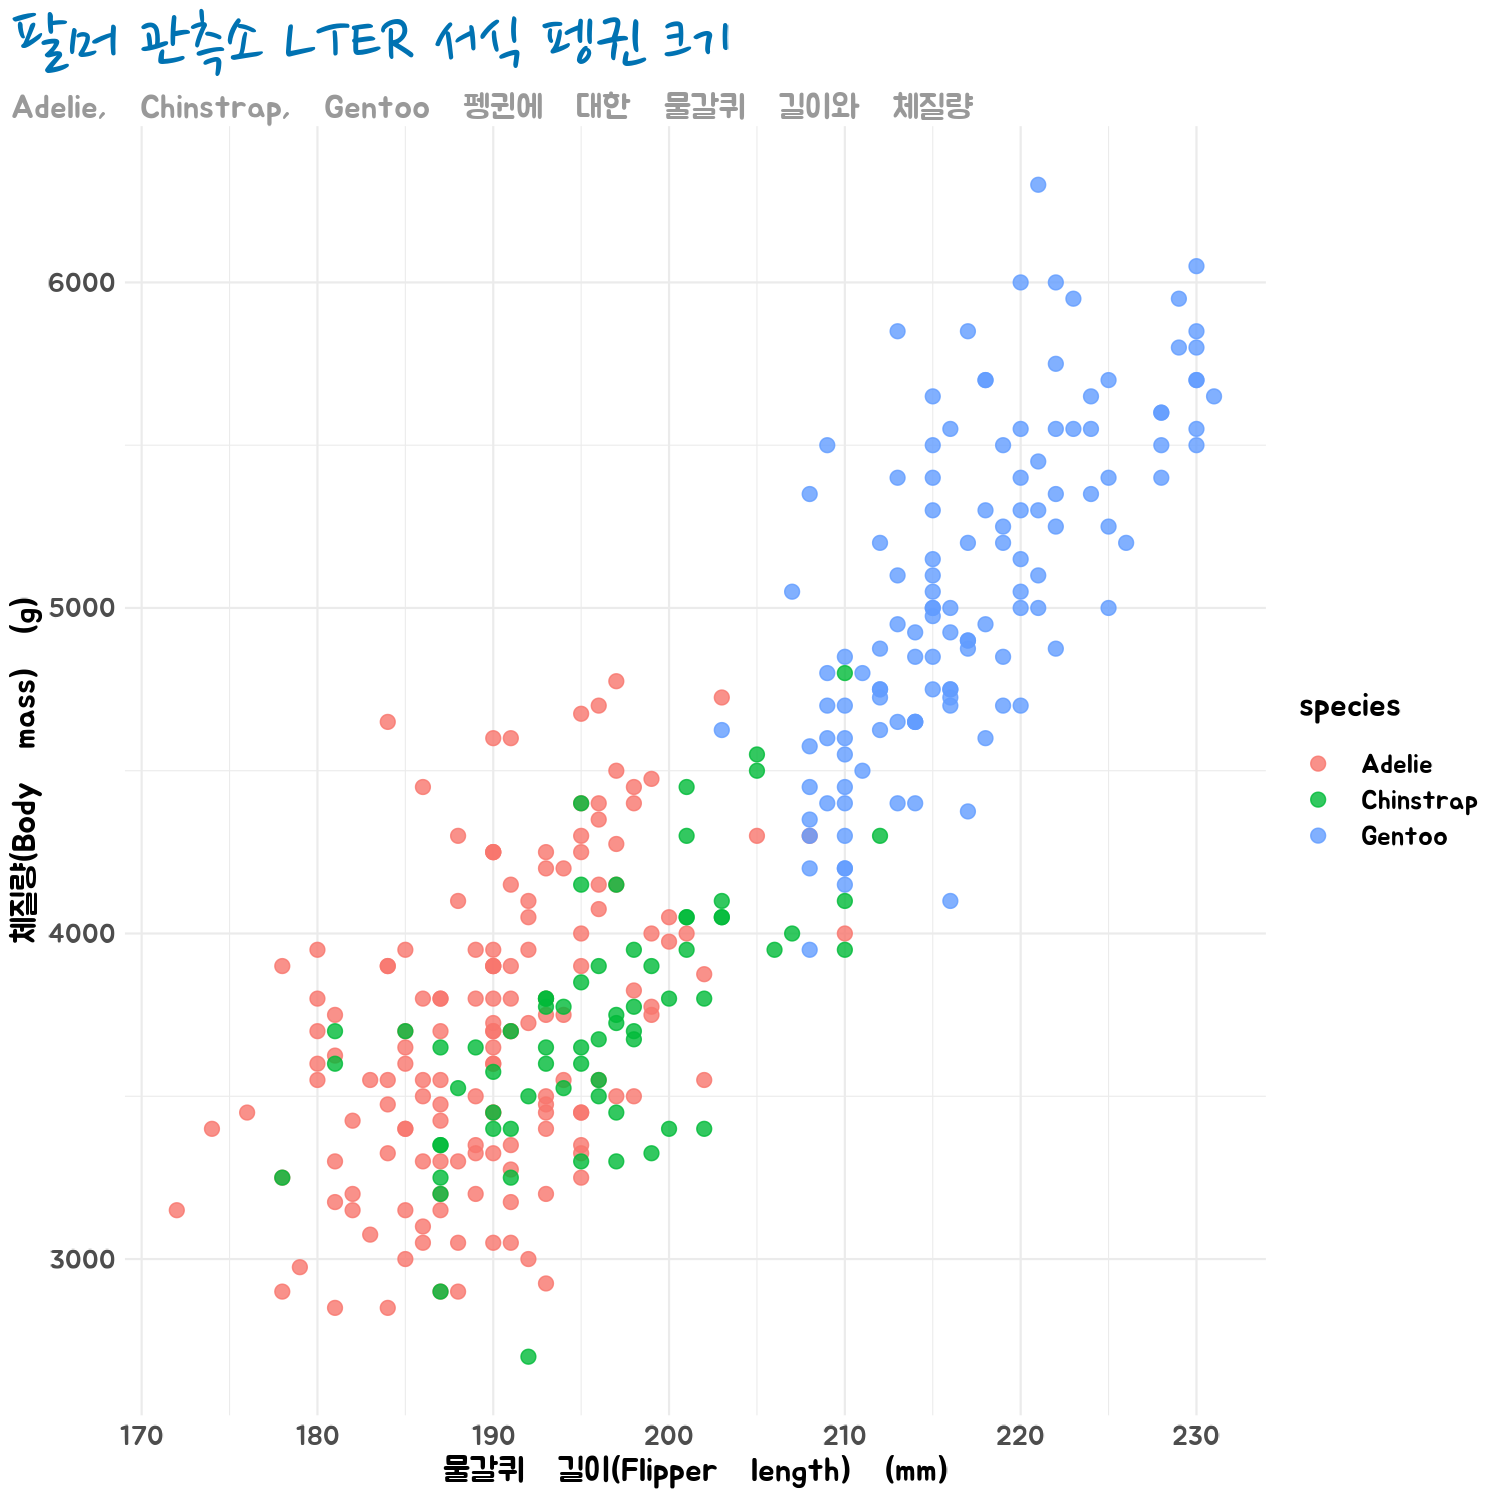
\includegraphics{images/penguins.png}

}

\caption{펭귄 시각화 사례}

\end{figure}

\hypertarget{uxcf54uxb4dc}{%
\section{코드}\label{uxcf54uxb4dc}}

\hypertarget{uxd30cuxc774uxc36c-uxcf54uxb4dc}{%
\subsection{파이썬 코드}\label{uxd30cuxc774uxc36c-uxcf54uxb4dc}}

\begin{Shaded}
\begin{Highlighting}[]
\BuiltInTok{print}\NormalTok{(}\StringTok{"파이썬에서 헬로 월드!"}\NormalTok{)}
\end{Highlighting}
\end{Shaded}

\begin{verbatim}
파이썬에서 헬로 월드!
\end{verbatim}

\hypertarget{r-uxcf54uxb4dc}{%
\subsection{R 코드}\label{r-uxcf54uxb4dc}}

\begin{Shaded}
\begin{Highlighting}[]
\FunctionTok{print}\NormalTok{(}\StringTok{"R에서 헬로 월드!"}\NormalTok{)}
\end{Highlighting}
\end{Shaded}

\begin{verbatim}
[1] "R에서 헬로 월드!"
\end{verbatim}

\hypertarget{uxc218uxc2dd}{%
\section{수식}\label{uxc218uxc2dd}}

간단한 수식을 보여줍니다:

\[
\int_0^\infty e^{-x^2} dx = \frac{\sqrt{\pi}}{2}
\]

\autocite{Smith2021}에서 언급한 것처럼 이것은 예시 문서입니다.

\hypertarget{uxae00uxc528-uxd06cuxae30}{%
\section{글씨 크기}\label{uxae00uxc528-uxd06cuxae30}}

Huge \textgreater{} huge \textgreater{} LARGE \textgreater{} Large
\textgreater{} large \textgreater{} normalsize \textgreater{} small
\textgreater{} footnotesize \textgreater{} scriptsize \textgreater{}
tiny

\Huge

쿼토(Quarto)가 글쓰기 미래다

\huge

쿼토(Quarto)가 글쓰기 미래다

\LARGE

쿼토(Quarto)가 글쓰기 미래다

\normalsize

쿼토(Quarto)가 글쓰기 미래다

\small

쿼토(Quarto)가 글쓰기 미래다

\footnotesize

쿼토(Quarto)가 글쓰기 미래다

\tiny

쿼토(Quarto)가 글쓰기 미래다

\normalsize

\hypertarget{uxb2e4uxc774uxc5b4uxadf8uxb7a8}{%
\section{다이어그램}\label{uxb2e4uxc774uxc5b4uxadf8uxb7a8}}

\begin{figure}[H]

{\centering 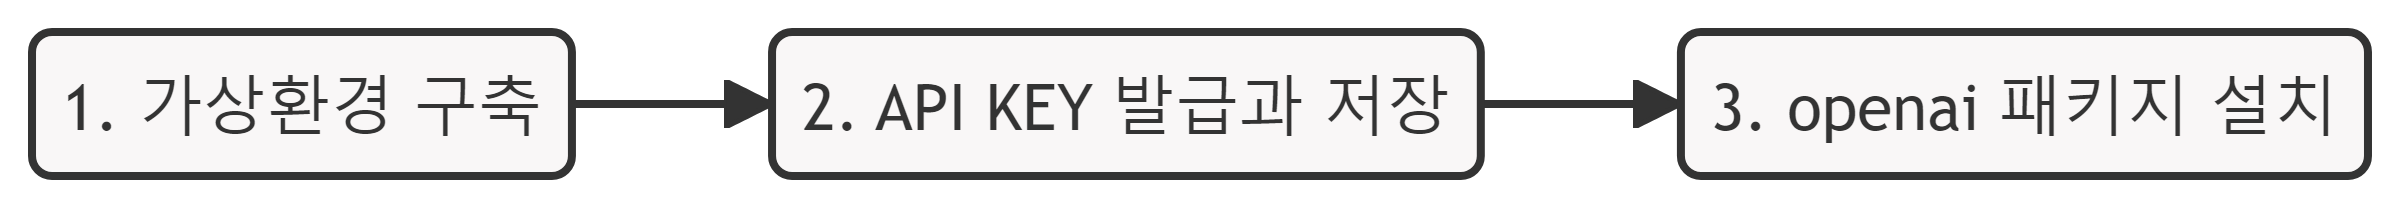
\includegraphics[width=6.25in,height=0.54in]{hello_quarto_files/figure-latex/mermaid-figure-1.png}

}

\end{figure}

\hypertarget{uxcc38uxace0uxbb38uxd5cc}{%
\section{참고문헌}\label{uxcc38uxace0uxbb38uxd5cc}}

참고 문헌 인용과 목록 생성 실험을
합니다.\index{참고 문헌}\index{인용}\index{citation} 한국어 문헌과
구미어 문헌은 그 목록형성과 인용 방법이 다릅니다. 한국어 문헌의 예를
들면, \autocite{kimuycwung_hankwukphan_2003}\과 같고, 영어 문헌은 예를
들면, \autocite{Allport:1992:OND}\과 같습니다.
\index{타당도}\index{신뢰도}\index{한국어 문헌}\index{korean}


\printbibliography[title=문헌목록]


\end{document}
